%% Font size %%
\documentclass[11pt]{article}

%% Load the custom package
\usepackage{Mathdoc}

%% Numéro de séquence %% Titre de la séquence %%
\renewcommand{\centerhead}{Chap. 2 : Points, droites, segments}

%% Spacing commands %%
\renewcommand{\baselinestretch}{1}
\setlength{\parindent}{0pt}

\begin{document}

\section{Points}
\begin{definition}
  En géométrie, un point est un objet sans taille ni dimension, souvent défini comme l'intersection de deux droites. Le point est défini uniquement par sa position.
\end{definition}

\begin{notation}
  \begin{enuspaced}  
  \item Il est représenté par une petite croix (un X) symbolisant
    l'intersection de deux droites.  
  \item Un point se note avec une lettre
    en majuscule.
  \end{enuspaced}
\end{notation}

\begin{exemple}
Soit A un point du plan : \\ \\
    \begin{tikzpicture}[scale=1.5]
      \tkzDefPoint(4,0){A} \tkzDrawPoints[shape=cross out](A)
      \tkzLabelPoints(A)
    \end{tikzpicture}
\end{exemple}

\section{Segments}

  \begin{definition}
    Un segment est l'ensemble des points alignés qui se situent entre
    le point A et le point B.
  \end{definition}

  \begin{vocabulaire}
    Les points A et B sont les extrémités de ce segment.
  \end{vocabulaire}
  
\begin{notation}
Ce segment se note $[AB]$ ou $[BA]$, sa longueur se note $AB$ ou $BA$.
\end{notation}

\begin{exemple}
  Soit $[AB]$ un segment d'extrémités A et B : \\
      \input{.figures/segment1.txt}
\end{exemple}

\section{Appartenance à un segment}

\begin{definition}
Si C est un point du segment $[AB]$, on dit qu'il appartient au segment. \\
On note $C\in [AB]$
\end{definition}

\begin{remarque}
Réciproquement, on note $D \notin [AB]$ pour D n'appartient pas à $[AB]$.
\end{remarque}

\newpage
\begin{exemple}
 Soit $[AB]$ un segment, avec $C \in [AB]$ et $D \notin [AB]$ : \\
      \input{.figures/segment2.txt}
  \end{exemple}

\section{Milieu d'un segment}

  \begin{definition}
    Le milieu d'un segment $[AB]$ est le point I, tel que :
    \begin{enu}
    \item $I \in [AB]$ (I appartient au segment)
    \item $IA=IB$ (I est à égale distance de A et de B)
    \end{enu}
  \end{definition}
  
  \begin{exemple}
    Soit $I$ le milieu du segment $[AB]$ : \\
      \input{.figures/segment3.txt}
  \end{exemple}

\section{Droites}

\begin{definition}
  Une droite est composée d'une infinités de points alignés entre eux.
\end{definition}

\begin{notation}
  On note une droite entre parenthèse, soit avec un couple de points
  (en majuscule), soit avec une lettre en minuscule.
\end{notation}

\begin{exemple}
Soit $(AB)$ la droite passant par les points A et B : \\
\begin{tikzpicture}

\tkzDefPoint(0,0){D}    
\tkzDefPoint(1,0){A}
\tkzDefPoint(6,0){B}
\tkzDefPoint(7,0){F}

\tkzDrawPoints[shape=cross out](A,B)

\tkzLabelPoints(A,B)

\tkzDrawSegments(D,F)

\tkzLabelSegment[sloped, above](A,B){$(AB)$}

\end{tikzpicture}
\end{exemple}

\begin{propriete}
  Par deux points on peut faire passer une droite et une seule : c'est-à-dire que deux points sont toujours alignés.
\end{propriete}

\section{Appartenance à une droite}

\begin{definition}
Si C est un point de la droite $(d)$, on dit qu'il appartient à cette droite. \\
On note $C\in (d)$
\end{definition}

\begin{exemple}
Ici, on a bien $C \in (d)$ : \\
\begin{tikzpicture} 
    
\tkzDefPoint(0,0){A}
\tkzDefPoint(3,3){B}
\tkzDefPoint(2,2){C}

\tkzDrawPoint[shape=cross out](C)

\tkzLabelPoints(C)

\tkzDrawSegments(A,B)

\tkzLabelSegment[sloped, above](A,B){$(d)$}

\end{tikzpicture}
\end{exemple}

\section{Demi-droites}

\begin{definition}
Une demi-droite est une portion de droite limitée d'un seul côté par un point.
\end{definition}

\begin{vocabulaire}
On appelle ce point, l'origine de la demi-droite.
\end{vocabulaire}

\begin{notation}
On note la demi-droite avec deux points, fermés par un crochet $[$
côté origine ; et une parenthèse $)$. 
\end{notation}

\begin{exemple}
Soit $[DE)$ la demi-droite d'origine $E$ : \\
\begin{tikzpicture}
    
\tkzDefPoint(0,0){D}
\tkzDefPoint(4,2){E}
\tkzDefPoint(6,3){F}

\tkzDrawPoints[shape=cross out](D,E)

\tkzLabelPoints(D,E)

\tkzDrawSegments(D,F)

\tkzLabelSegment[sloped, above](D,E){$[DE)$}
\end{tikzpicture}
\end{exemple}

\begin{remarque}
Un point appartenant à la droite $[AB]$, n'appartient pas
nécessairement à la demi-droite $(AB]$.
\end{remarque}


\begin{exemple}
  $C \in (AB)$ mais $C \notin (AB]$ :
  
\begin{tikzpicture}
    
\tkzDefPoint(2,1){A}
\tkzDefPoint(4,2){B}
\tkzDefPoint(5,2.5){C}
\tkzDefPoint(0,0){D}
\tkzDefPoint(6,3){F}

\tkzDrawPoints[shape=cross out](A,B,C)

\tkzLabelPoints(A,B,C)

\tkzDrawSegments(D,F)

\tkzLabelSegment[sloped, above](D,F){$(AB]$}
\end{tikzpicture}
\end{exemple}


\end{document}

%%% Local Variables:
%%% mode: LaTeX
%%% TeX-master: t
%%% End:
